\section{Designing a multi-channel BT scanner}
\label{sec:hyperscanner:design}

\subsection{A multi-channel Bluetooth scanning protocol}
As discussed in section~\ref{sec:hyperscanner:bkgd}, conventional Bluetooth scanning using narrowband scanner (e.g. smartphone) can take from 10.96s -- 40.96s, which is very slow for wardriving applications.
%
This slow speed is a consequence of the sequential nature of transmitting ID packets, and the fact that the Bluetooth devices are sleeping for majority of their time.
%

We define a new fast multi-channel scanning protocol, that can be implemented on  wideband SDRs.
%
The following key insights help us define this faster scanning protocol:
\begin{enumerate}
    \item If a Bluetooth device is awake and hears an ID packet, it will reliably respond with a FHS packet exactly 625$\mu$s later.
    \item A Bluetooth device will listen for ID packets for 11.25ms in a 1.28s duration.
\end{enumerate}
\begin{figure}
    \centering
    \captionsetup{justification=centering}
    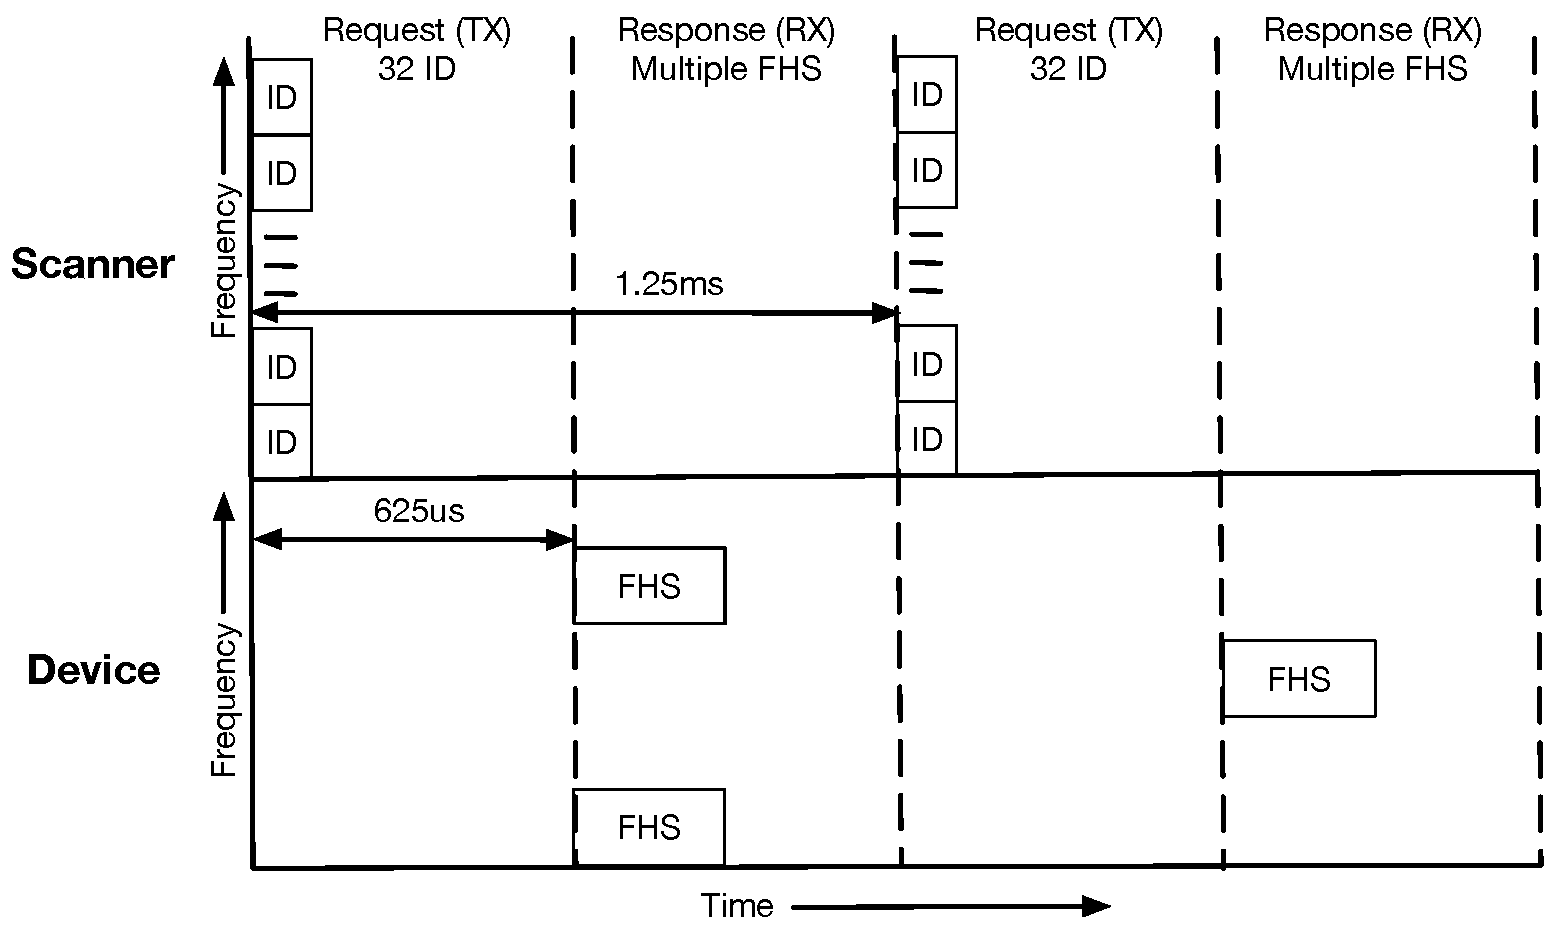
\includegraphics[width=\textwidth]{hyperscanner/figs/bt_multi_chain.pdf}
    \caption{Multi-channel scan process and timing}
    \label{fig:hyperscanner:bt_multi_chan}
\end{figure}

Instead of a train of ID packets spread over 10ms, we transmit ID packets on all channels in a burst at the start of every request time slot, using the TX chain of the SDR.
%
Figure~\ref{fig:hyperscanner:bt_multi_chan} shows the packet transmissions and timing for this new scanning process.
%
We ensure tight timing control to ensure that the next burst is transmitted exactly two slots later (1.25ms later). 
%
Every Bluetooth device that is listening, will respond back with a FHS packet at the start of the response time slot. 
%
These packet signals can be received by the wideband RX chain of our SDR, and decoded to obtain the relevant auditing information.
%

We need to repeat this burst a certain number of times to ensure every sleeping device wakes up and responds.
%
Since typical Bluetooth devices wake up once in a 1.28s interval (for 11.25ms interval), repeating the bursts for a duration of 1.28s should ensure we are able to get responses from every surrounding device.
%
In a noisy environment, we may need to repeat these bursts for double the time, or 2.56s. 
%
This is significant theoretical improvement over the scanning speed possible with conventional scanning tools.

\subsubsection*{Handling PAPR issues}
While our ID packet burst strategy improves the scanning speed, we cannot use this packet burst directly on SDR hardware.
%
In particular, ID packets have the exact same packet contents, resulting in the same waveform being transmitted on all frequency channels at the exact same time instant.
%
This results in the overall wideband signal having pulses in the time domain, which is problematic for the analog hardware of our SDR.
%
These pulses result in a very high Peak-to-Average-Power-Ratio (PAPR), and these get significantly distorted due to non-linearities of the programmable amplifier (PA).
%
In addition, high PAPR signals are difficult to represent using the limited resolution of the DACs.
%
This PAPR problem is commonly encountered with radios transmitting OFDM signals, which is very similar to the multi-channel ID packets burst for our scenario.

To reduce the PAPR of the overall wideband signal, we stagger the ID packets on consecutive frequency channels by a small time duration. 
%
This breaks the frequency repetition, and prevents formation of pulses in time domain.
%
We offset each channel's packet in time by a $N*t_{stagger} \mu$s, where $N$ is the frequency channel index.
%
Figure~\ref{fig:hyperscanner:stagger} qualitatively shows how our staggering the ID packets reduces the peak power of the signal, making it more amenable to transmission without distortion.
%
\begin{figure}[!h]
    \centering
    \begin{subfigure}{0.48\textwidth}
        %\centering
        %\captionsetup{justification=centering}
        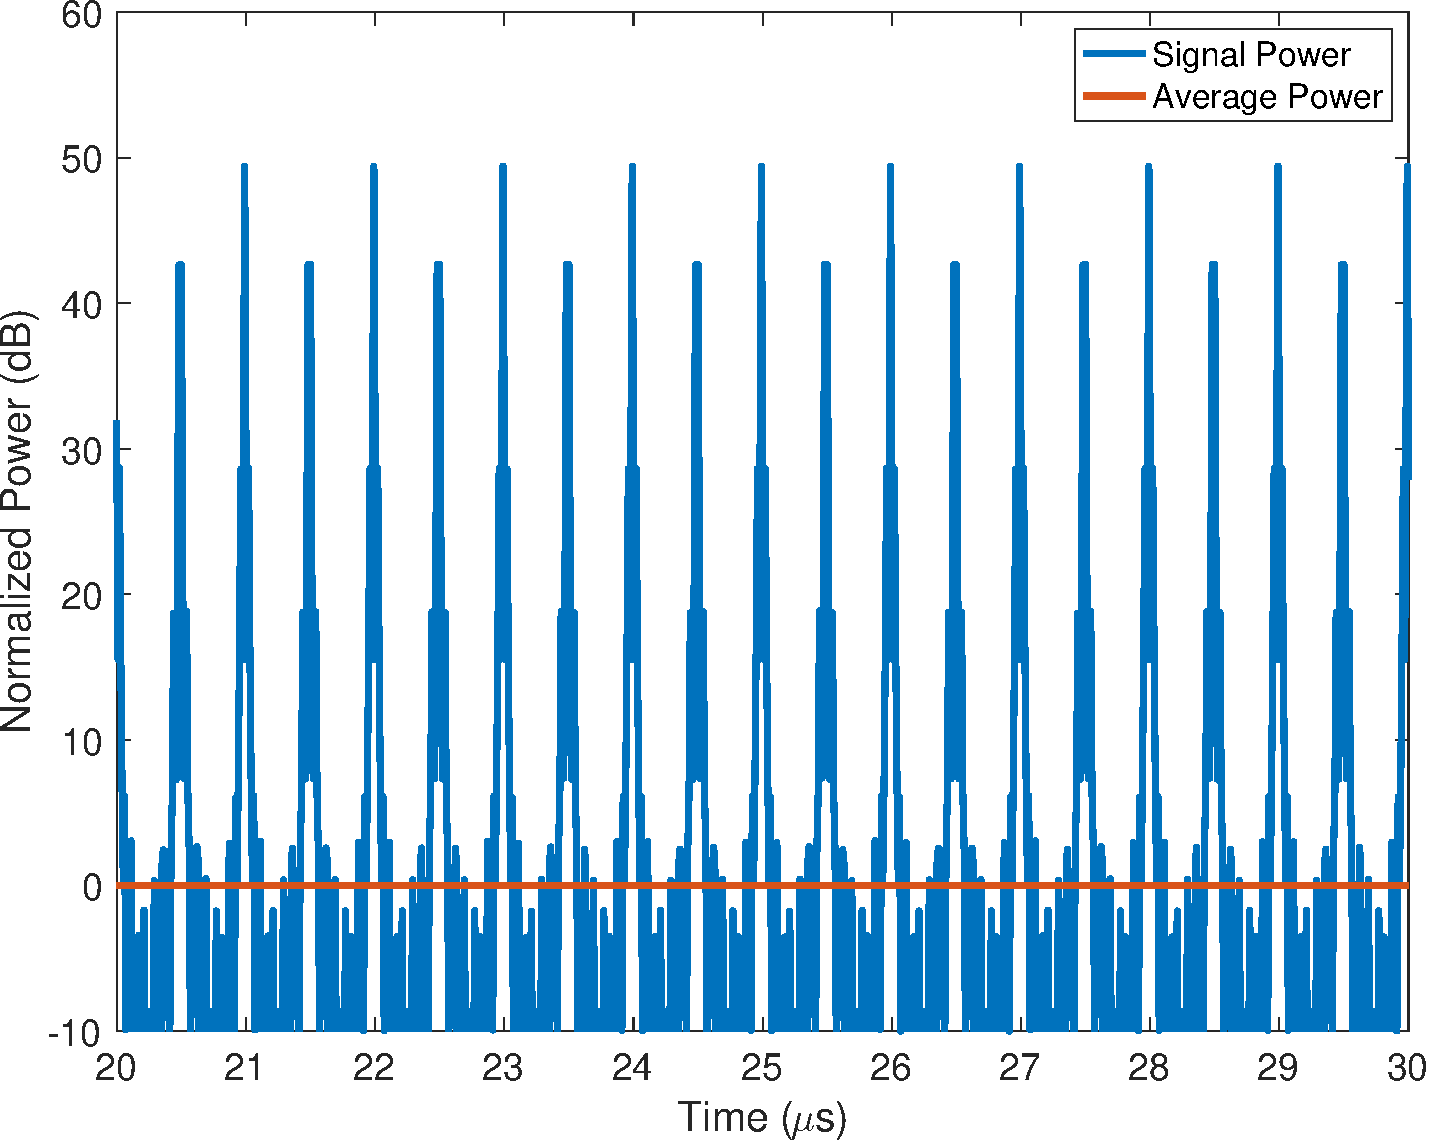
\includegraphics[width=\textwidth]{hyperscanner/plots/power_single_bt.pdf}
        \caption{}
        %\label{fig:hyperscanner:bt_multi_chan}
    \end{subfigure}
    \hfill
    \begin{subfigure}{0.48\textwidth}
        %\centering
        %\captionsetup{justification=centering}
        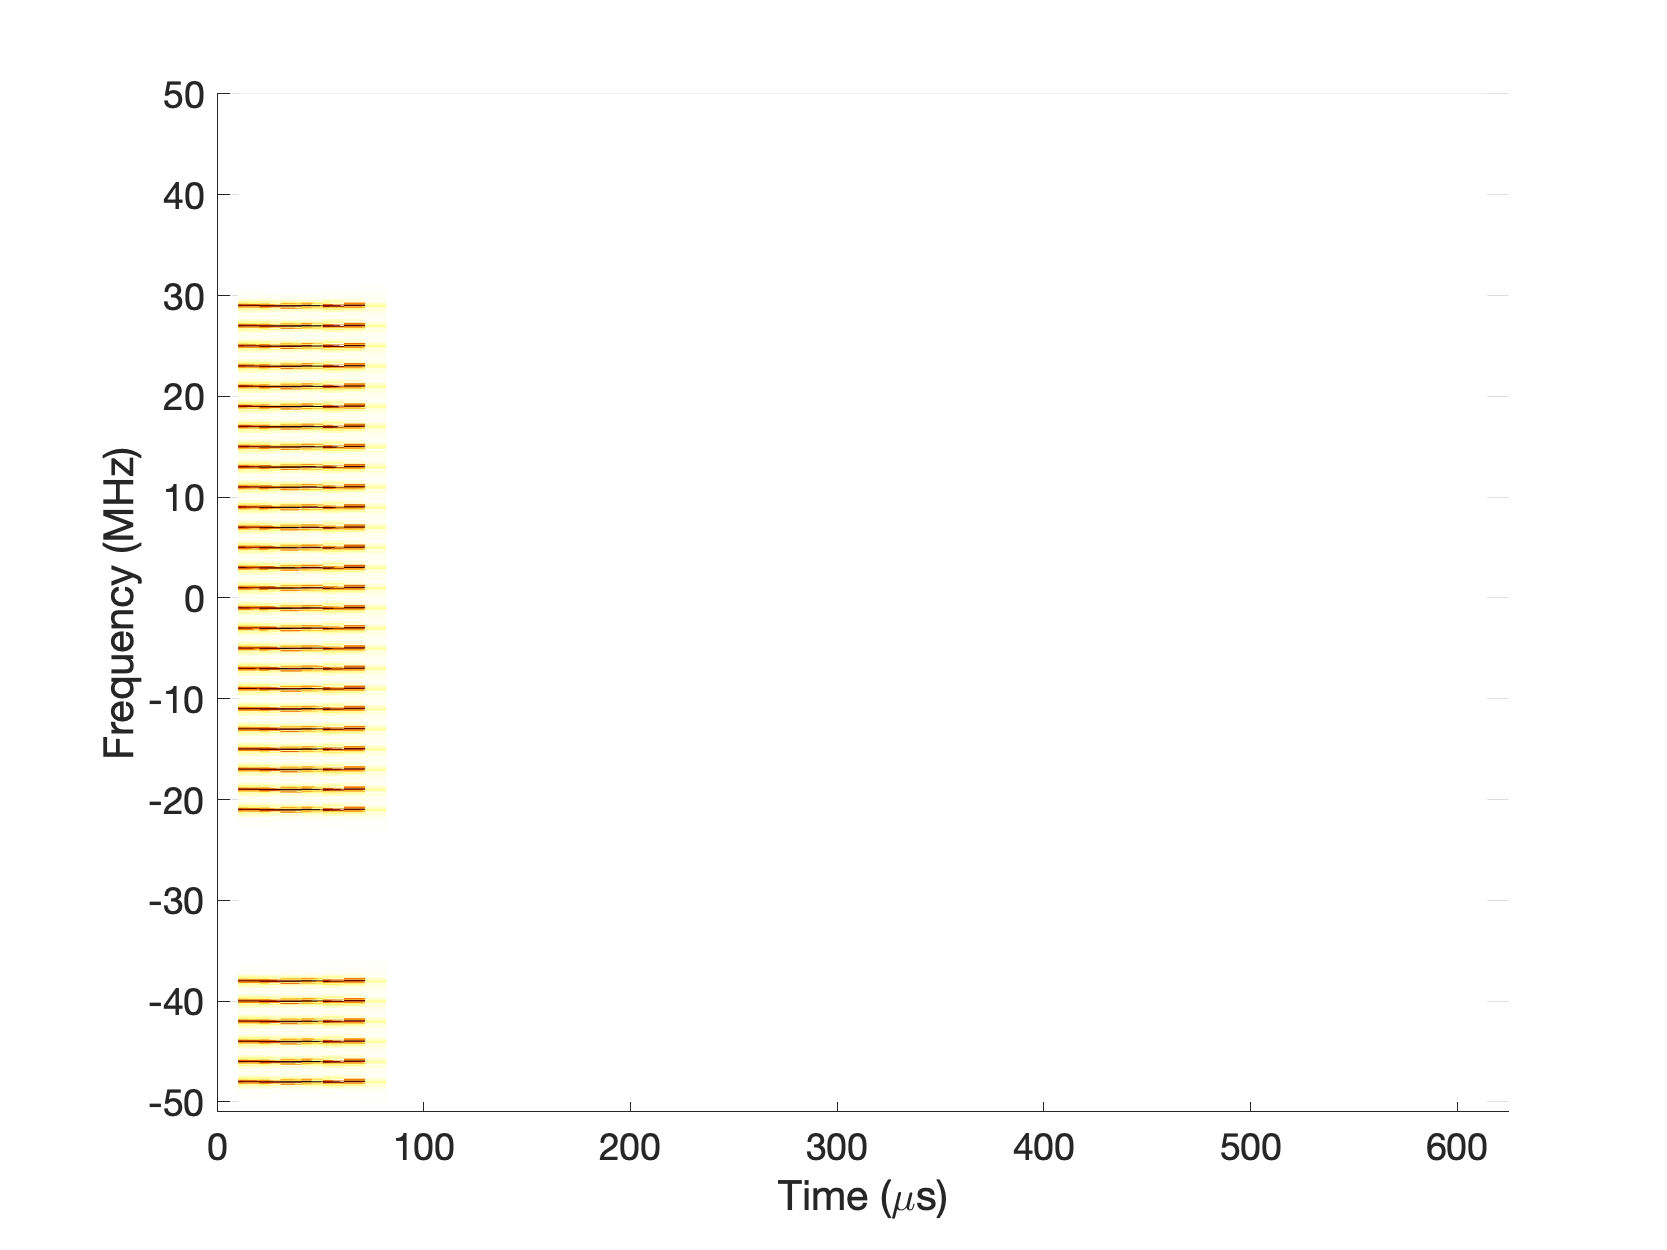
\includegraphics[width=\textwidth]{hyperscanner/plots/stft_single_bt2.pdf}
        \caption{}
        %\label{fig:hyperscanner:bt_multi_chan}
    \end{subfigure}
    \medskip
    \begin{subfigure}{0.48\textwidth}
        %\centering
        %\captionsetup{justification=centering}
        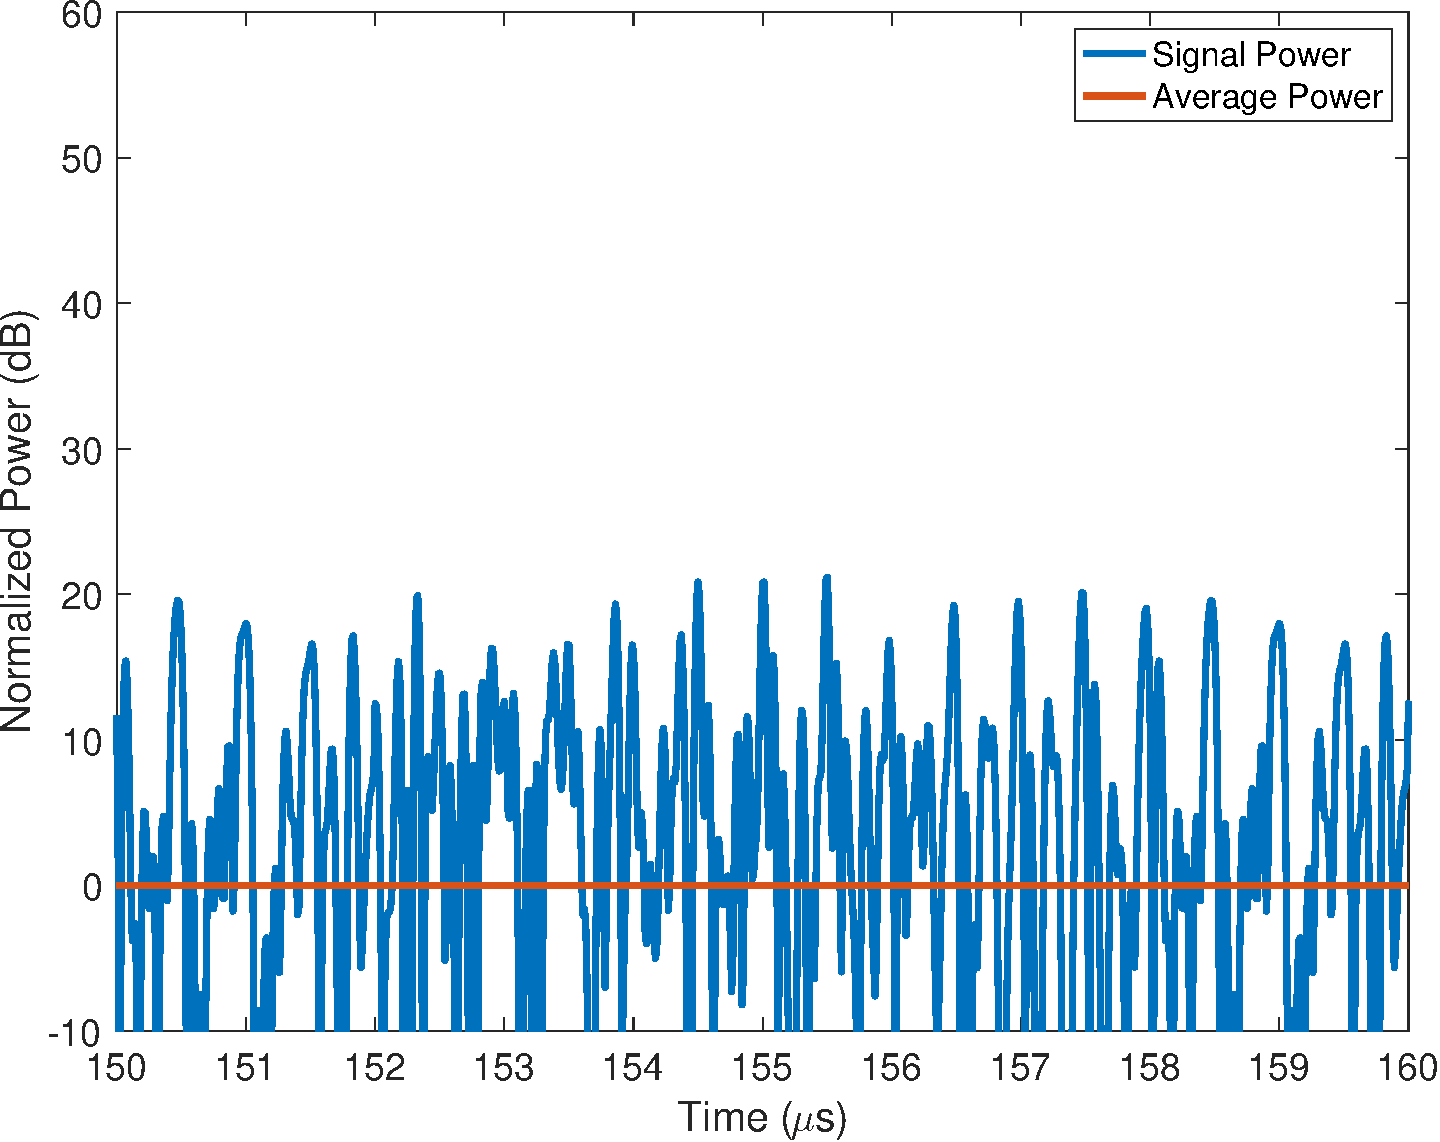
\includegraphics[width=\textwidth]{hyperscanner/plots/power_multi_bt.pdf}
        \caption{}
        %\label{fig:hyperscanner:bt_multi_chan}
    \end{subfigure}
    \hfill
    \begin{subfigure}{0.48\textwidth}
        %\centering
        %\captionsetup{justification=centering}
        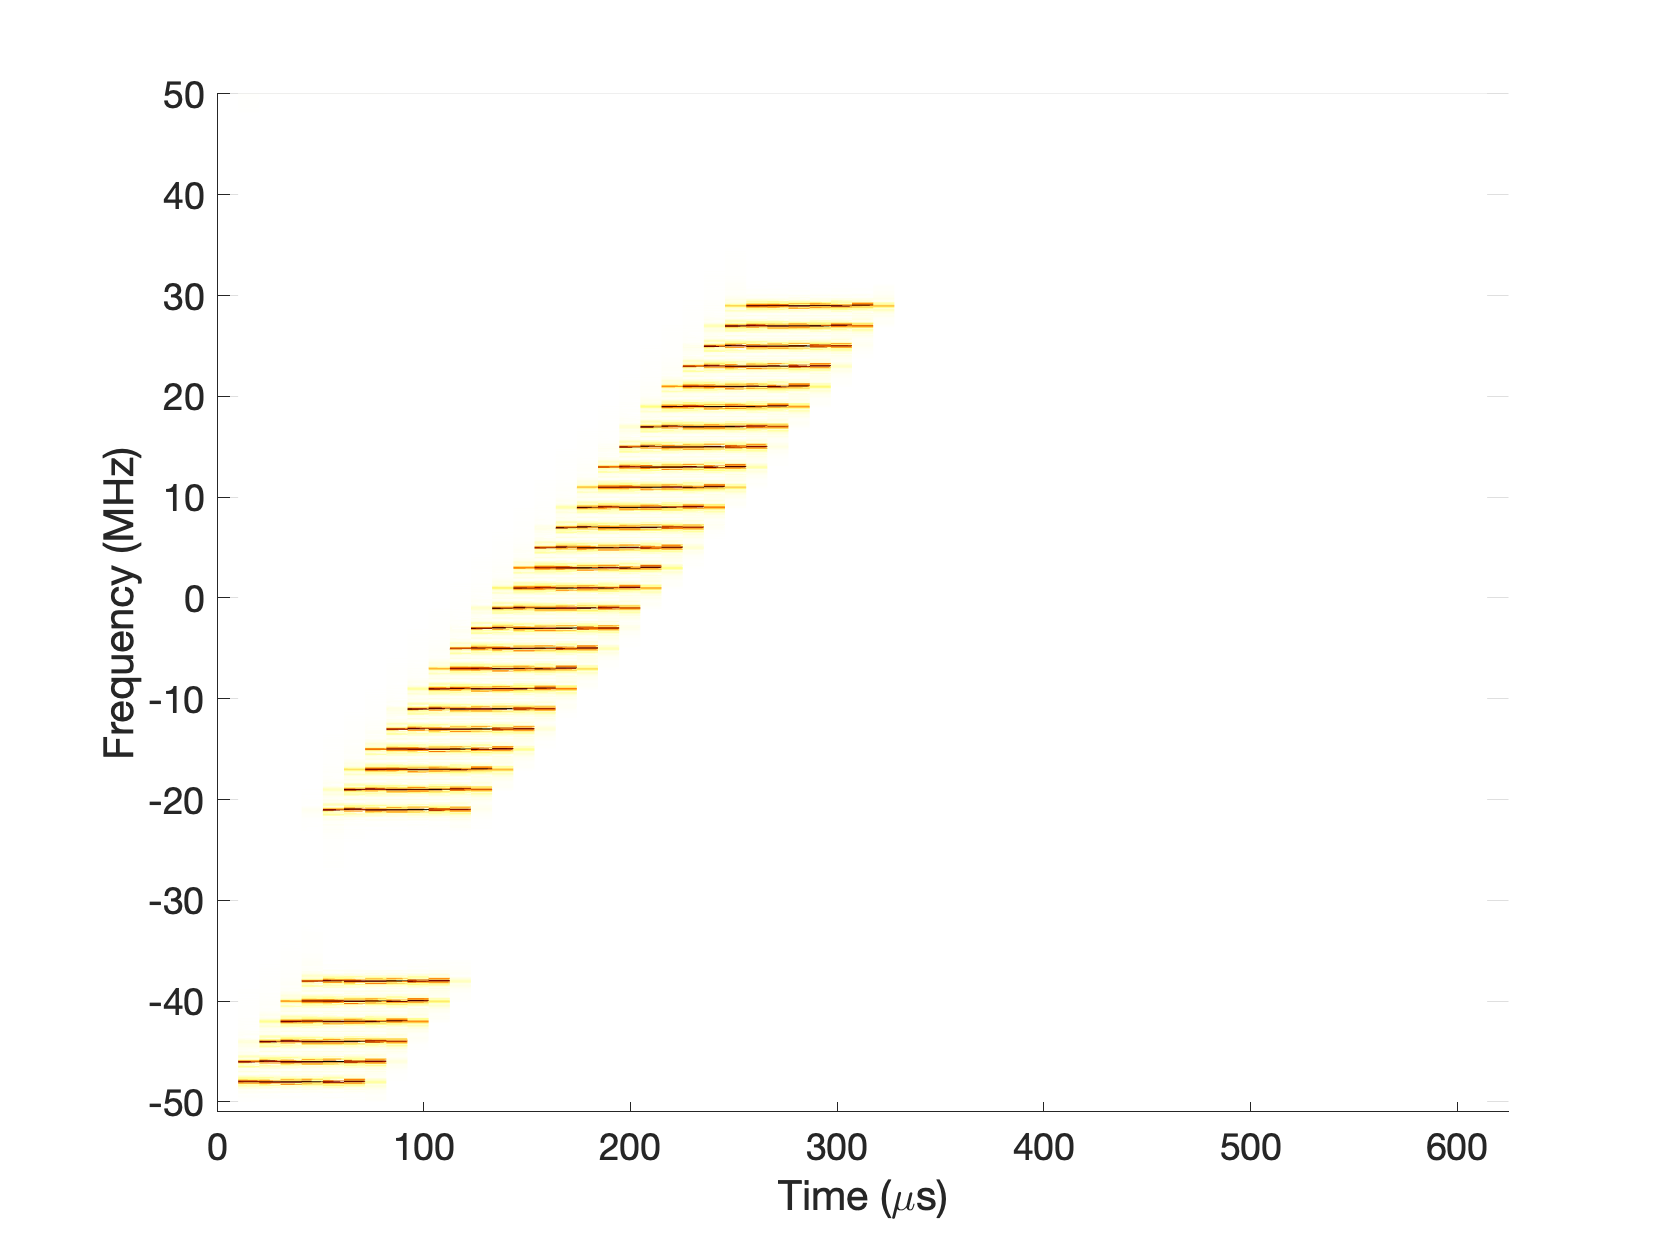
\includegraphics[width=\textwidth]{hyperscanner/plots/stft_multi_bt2.pdf}
        \caption{}
        %\label{fig:hyperscanner:bt_multi_chan}
    \end{subfigure}
    \captionsetup{justification=centering}
    \caption{Reducing PAPR by staggering ID packets. Subfigures (a) and (c) show the time domain wideband signal with and without the stagger, and (b) and (d) are the spectral plots showing the time shift of consecutive ID packets. The peak power is significantly reduced with the stagger.}
    \label{fig:hyperscanner:stagger}
\end{figure}

The value of $t_{stagger}$ is chosen with a few considerations. 
%
Firstly, most radios are designed to handle PAPR of 15dB. 
%
We choose a stagger time to bring the PAPR of the signal below 15 dB and ensure that the quantization noise is minimized. 
%
Secondly, the value of time offset should be such that we can maintain the tight request and response slot boundaries.
%
FHS responses are received exactly $625\mu$s after ID packets and a typical FHS packet is $366\mu$s in length.
%
In order to ensure that we can receive this FHS response within the $625\mu$s response slot boundaries, our stagger time must be so that the last ID packet is transmitted $\leq259\mu$s.
%
This can be done for a $t_{stagger}\leq8.35\mu$s.
In Figure~\ref{fig:hyperscanner:papr_stagger}, we show the relationship between $t_{stagger}$ and the PAPR. 
%
$t_{stagger}=8.2 \mu$s is chosen for our system, as it gives the lowest PAPR within the constraints mentioned above.
%
\begin{figure}[h!]
    \centering
    \captionsetup{justification=centering}
    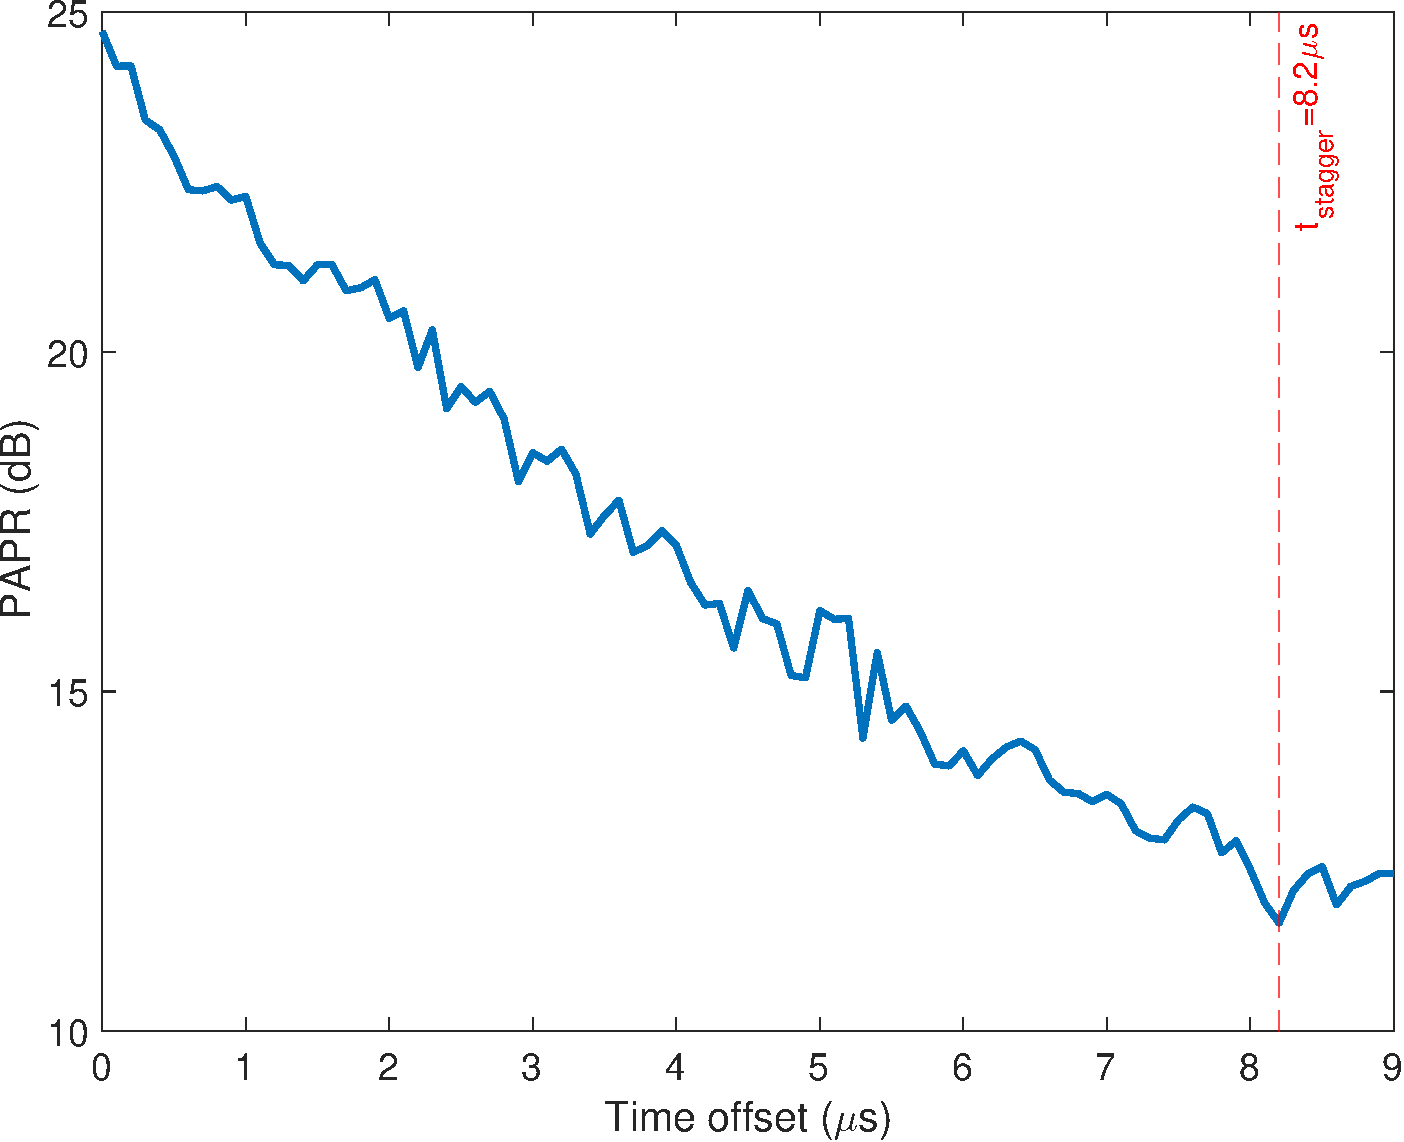
\includegraphics[width=0.6\textwidth]{hyperscanner/plots/papr_stagger.pdf}
    \caption{Variation of PAPR with the stagger time offset of ID packet burst. Dotted line shows the chosen stagger value for our system}
    \label{fig:hyperscanner:papr_stagger}
\end{figure}

\subsection{Multi-channel scanning on low-end commodity SDR}
Implementation of the multi-channel scanning protocol requires a hardware platform that supports a wide analog bandwidth to cover the entire 76 MHz band, on both transmit and receive sides.
%
It also should have processing capability to process raw FHS signals at any response frequency, decode and extract information from the FHS packets.
%
There are several commodity SDR platforms, e.g. USRP x300, that support a wide analog bandwidth (upto 160 MHz), and a large network bandwidth (10Gbps ethernet link) to offload processing on a separate computer. 
%
But such platforms costs several thousand dollars and need a separate computer for processing and decoding, making them not portable or scalable and therefore unsuitable for large scale empirical wireless auditing.

Instead, we chose to implement our system on the Analog Devices ADALM-PLUTO (PlutoSDR) software radio. 
%
The PlutoSDR is a popular example of a new class of modern SDRs -- low-cost, standalone units with on-board processing capability. 
%
It costs only \$230 and includes analog front-end(filter, amplifiers), ADCs, DACs, FPGA as well as an ARM processor (667 MHz dual-core) and 512 MB memory. 
%
The processor on the Pluto runs Linux and can support on-board custom signal processing and packet decoding. 
%
The PlutoSDR is an ideal platform in terms of cost and portability to implement our wardriving scanning tool.
%

However, there are certain hardware challenges that we have to overcome for using the PlutoSDR for our multi-channel Bluetooth scanning tool.
%
Firstly, the Pluto has a limited analog bandwidth of 56 MHz on the receive side and 40 MHz on the transmit side. 
%
Since the Bluetooth request and response channels are spread across a 76 MHz band, the PlutoSDR will be unable to send ID packets and receives FHS packets across the entire Bluetooth band.
%
Second, even for the response channels it can sense, PlutoSDR's sampling rate of 61.44 million samples per second results in 245 MB of sample data per second on the receive side. 
%
The built-in processor is not powerful enough to filter and decode in real-time this large amount of data.
%
In the following subsections, we provide some initial ideas on overcoming these hardware design challenges.

\subsubsection{Extending the analog bandwidth}
Classic Bluetooth has request channels spread across 76 MHz (2.402 GHz -- 2.477 GHz), and response channels spread across 63 MHz (2.414 GHz -- 2.476 GHz).
%
However, PlutoSDR only supports an analog bandwidth of 56 MHz on transmit side, and 40 MHz on receive side, resulting in some Bluetooth channels being out-of-band.
%
As a consequence, the PlutoSDR won't be able to query and listen on all channels which will result in an unwanted increase in scan time.
%
\begin{figure}[h!]
    \centering
    \captionsetup{justification=centering}
    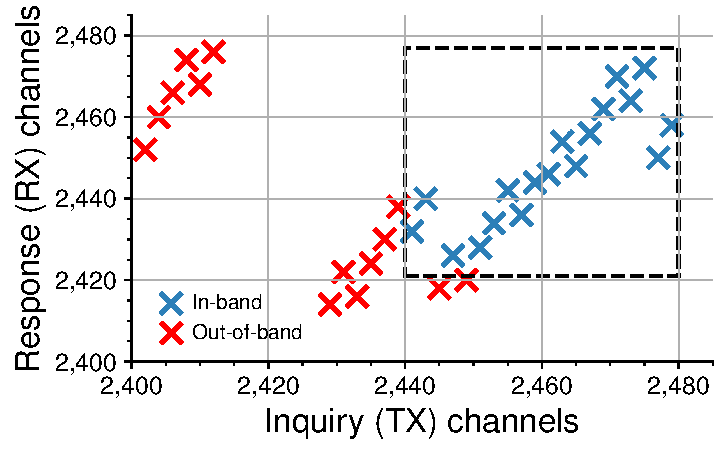
\includegraphics[width=0.6\textwidth]{hyperscanner/plots/inq_resp_og.pdf}
    \caption{Map of request/response channels showing out-of-band channels for PlutoSDR. The dotted lines represent the analog bandwidth limits of the Pluto.}
    \label{fig:hyperscanner:outofband}
\end{figure}

To extend the analog bandwidth of the Pluto, a key insight comes from how request/response channels are distributed in the 2.4GHz band. 
%
Request and response channels are interspersed across the band, and the time slotted ALOHA nature of Bluetooth scanning means that request channels are free during response time slots and vice-versa.
%
Therefore,
during response slot if we can create an image of the out-of-band
channels onto the free in-band channels, we can easily receive those
responses. 
%
Similarly, in inquiry slot we can transmit on the free
in-band channels and create images onto the necessary out-of-band
inquiry channels.
%
Figure~\ref{fig:hyperscanner:unusedchans} demonstrates this idea.

\begin{figure}[h!]
    \centering
    \captionsetup{justification=centering}
    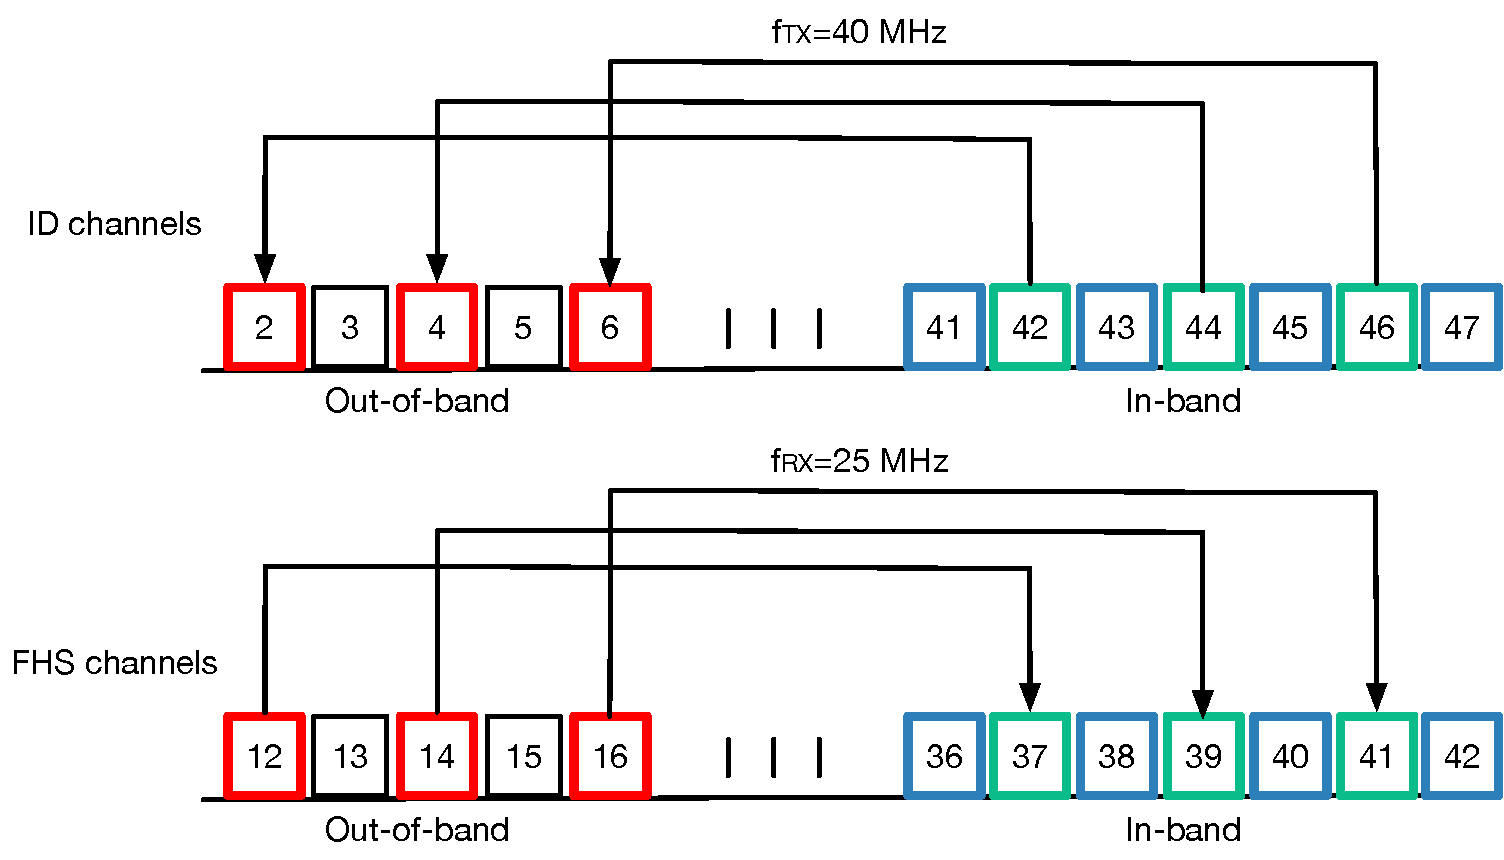
\includegraphics[width=0.8\textwidth]{hyperscanner/figs/switch_channels.pdf}
    \caption{Utilizing unused request and response channels for moving out-of-band channels in-band and vice versa}
    \label{fig:hyperscanner:unusedchans}
\end{figure}

To create these images, we can use an analog frequency mixer.
%
However, that would require us to generate the appropriate frequency shifts using an additional voltage controlled oscillator, increasing the system cost and complexity.
%
Instead, for our design we utilized an RF switch as a mixer(cite backscatter papers) and generate the necessary TX and RX shifting frequencies (switch control input) directly from the PlutoSDR's FPGA.
%
We use a shift frequency $f_{TX}=40$MHz for ID packets, and $f_{RX}=25$MHz for FHS packets. 
%
On the transmit side, the use of a square wave as a switch input will generate harmonics even outside the 2.4GHz. We use a 2.4 GHz band filter to remove these unwanted images.
%
Figure~\ref{fig:hyperscanner:bwextend} shows our system block diagram and the remapped inquiry and response channels in our final system hardware.
%
\begin{figure}[h!]
    \centering
    \begin{subfigure}{0.4\textwidth}
        %\centering
        %\captionsetup{justification=centering}
        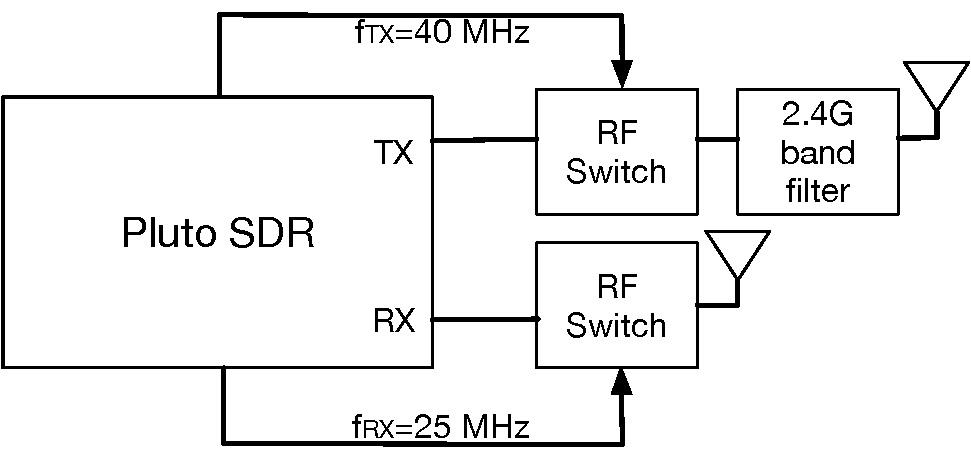
\includegraphics[width=\textwidth]{hyperscanner/figs/system_design.pdf}
        \caption{}
        %\label{fig:hyperscanner:bt_multi_chan}
    \end{subfigure}
    \hfill
    \begin{subfigure}{0.55\textwidth}
        %\centering
        %\captionsetup{justification=centering}
        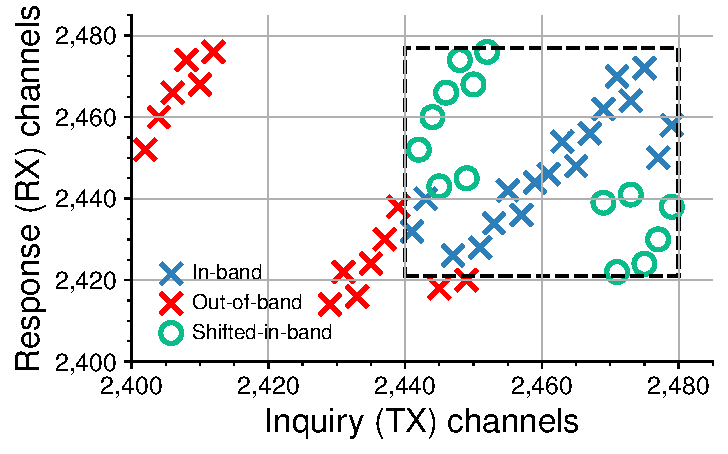
\includegraphics[width=\textwidth]{hyperscanner/plots/inq_resp_shifted.pdf}
        \caption{}
        %\label{fig:hyperscanner:bt_multi_chan}
    \end{subfigure}
    \captionsetup{justification=centering}
    \caption{Extending the analog bandwidth of PlutoSDR. (a) shows the system block diagram and (b) shows the new map of request/response channels with shifted images}
    \label{fig:hyperscanner:bwextend}
\end{figure}

\subsubsection{Minimizing data backhaul using SparSDR}
The PlutoSDR needs to listen for responses on channels spread across a wideband (56 MHz). 
%
Typically, this is done by running the analog to digital converters at a very high sampling rate (61.44 Msps), receive the raw signal samples, and then decode them per channel to obtain the Bluetooth device information (MAC address, device type).
%
Unfortunately, this high sampling rate will result in almost 245 MB of raw sample data that needs to be processed. 
%
The PlutoSDR processor is not powerful enough to this in real-time, nor does it have sufficient on-board memory to store this temporarily.
%
Worse, the majority of this compute is unnecessary because (1) the response channels only occupy 32 MHz of the total receive bandwidth, and (2) FHS packets are not received all the time, most of the time we only get useless signals or noise. 
%

To solve this problem, we utilized our previous project SparSDR. SparSDR provides the ability to compress the spectrum in both frequency and time. 
%
It lets us channelize the spectrum by masking out the frequency channels which are unused, allowing us to only receive signals in the 32 MHz of actual response channels. 
%
Additionally, it lets us threshold the signal level in the individual channels, ensuring that we only need to spend time processing signals that are above a certain power level, and not waste resources processing noise samples.
%
Coupled with the fact that actual spectrum occupancy is very low  even in noisy environments, SparSDR helps us drastically reduce the amount of data the processor needs to handle.
%
The processor now only needs to process when there are valid signals above a certain power on the response channels.